\documentclass[11pt, headings=normal]{scrartcl}

\usepackage{geometry}                % See geometry.pdf to learn the layout options. There are lots.
\geometry{a4paper}                   % ... or a4paper or a5paper or ... 

%%%%%%%%%%%biblatex setup%%%%%%%%%%
\usepackage[%
natbib=true, %allows natbib style citation commands
style=authoryear,%authoryear citation/bibliographic style
isbn=false, %don't show ISBNs
url=true, %do show urls where appropriate
doi=false, %don't show DOIs
eprint=false,%no print field
sortlocale=en, %sort bib entries in English order
firstinits=true, %makes bib forenames into initials
urldate=long, %affects format of URL access date 
dateabbrev=true% makes sure above uses short month names
]{biblatex}

\DeclareNameAlias{sortname}{last-first}%all author names surname first

%%%%%%%FORMATTING CITATIONS%%%%%

\DeclareFieldFormat{postnote}{#1}%gets rid of pp. in citations
\renewcommand{\nameyeardelim}{~}% just a space, no comma, between name and yr in citations
\renewcommand{\postnotedelim}{:\,}% colon+narrow space before pages in citations
\renewcommand{\intitlepunct}{\,}% gets rid of colon after 'In' in collected works

%%%%%%%%%%%%%%%%%

%%%FORMATTING BIBLIOGRAPHY LISTING%%%%%%

\renewbibmacro{in:}{%suppresses "In:" ...
  \ifentrytype{article}{}{%if its an article
  \printtext{\bibstring{in}\intitlepunct}}}

\DeclareFieldFormat
  [article, inbook, incollection, inproceedings, patent, thesis, unpublished]
  {title}{#1}%no quotes around titles of chapters/article titles

\DeclareFieldFormat
  [article, inbook, incollection, inproceedings, patent, thesis, unpublished]
  {volume}{\mkbibparens{#1}\nopunct} %puts volume number in brackets

\DeclareFieldFormat
  [article, inbook, incollection, inproceedings, patent, thesis, unpublished]
  {number}{{#1}\addcolon} % issue number followed by colon

\DeclareFieldFormat
  [article, inbook, incollection, inproceedings, patent, thesis, unpublished]
  {pages}{{\nopp#1}} %removes 'pp.' from pages
  
\DefineBibliographyStrings{english}{%
urlseen = {Accessed:},% What goes in front of the date a URL was accessed/retrieved et
editor = {(Ed)},%Ed - no dot, in brackets
editors = {(Eds)},% Eds - no dot, in brackets
byeditor = {(Ed.)}}% 'Edited by' for edited volumes

%\DefineBibliographyStrings{english}{in = {\,}}% What to use for 'IN'

%%%%%%%%%end of bib latex setup%%%%%%%%%%%%

\addbibresource{/Users/spkb/Dropbox/Bibliographies/mybib-noj.bib}

\usepackage{graphicx}
\usepackage{epstopdf}
\usepackage{filecontents}% allows data in source file
\usepackage{xcolor}%color for bar graphs
\usepackage{pstricks}%for drawing graphs etc
\usepackage{pst-bar}%for drawing bar graphs
\usepackage{pst-plot}%for drawing plotted lines
\usepackage{pstricks-add}%as above - needs to be last

\usepackage[linecolor=red, backgroundcolor=white, bordercolor=red]{todonotes}%todos in margin
\usepackage{textcomp}%text goodies

\usepackage{tabulary}% necess for MMD - tables
\usepackage{booktabs}% necess for MMD - tables
\usepackage{hyperref}% necess for MMD - Xref system
\usepackage[nameinlink, noabbrev]{cleveref}

\usepackage{xspace}
\newcommand{\hb}{\emph{hanbaiten}\xspace}
\newcommand{\og}{\emph{oshigami}\xspace}
\newcommand{\crs}{\emph{chirashi}\xspace}
\newcommand{\nnip}{\emph{Niigata Nippō}\xspace}
\newcommand{\ty}{\textyen}

\hyphenation{te-re-bi}

%%%create CJK cmd and env for Japanese text%%%%%%%%%%%%%%
\usepackage{fontspec}
 \defaultfontfeatures{Scale=MatchLowercase}
\newenvironment{CJK}{\fontspec[Scale=0.9]{Hiragino Mincho Pro}}{}
\newcommand{\cjk}[1]{{\fontspec[Scale=0.9]{Hiragino Mincho Pro}#1}}
%%%%%%%%%%%%%%%%%%%%%%%%%%%%%%%%%%%%

\DeclareGraphicsRule{.tif}{png}{.png}{`convert #1 `dirname #1`/`basename #1 .tif`.png}
\XeTeXlinebreaklocale"en"%enables Japanese text/line breaking

%\renewcommand\enoteformat{% this formats the endnotes without superscript numbers
%   \noindent\theenmark.\ \hangindent .7\parindent%
%}
%%%%%%%NEW LIST ENVIRONMENTS%%%%%%%%%%%
\newenvironment{close_enum}{
\begin{enumerate}
 \setlength{\itemsep}{1pt}
 \setlength{\parskip}{1pt}
 \setlength{\parsep}{0pt}}{\end{enumerate}
}
\newenvironment{close_descrip}{
\begin{description}
 \setlength{\itemsep}{1pt}
 \setlength{\parskip}{1pt}
 \setlength{\parsep}{0pt}}{\end{description}
}
%%%%%%%%%%%%%%%%%%%%%%%%%%%%%%%%%%%
\begin{document}

\def\mytitle{Interpretation of camera angles in television news}
\def\myauthor{Scott Koga-Browes}
\title{\mytitle}%TITLE OF PAPER
\author{\myauthor}%AUTHOR oF PAPER
\date{}%LEAVE BLANK FOR TODAY'S DATE
\maketitle

\begin{abstract}
\label{abstract}
\noindent
This study compares the portrayal of individuals in television news in terms of the camera angles used.

I look at both vertical camera angles, a semiotic resource theoretically used to express meanings of power and authority, and horizontal camera angles, seen as an indicator of ‘engagedness’.

An analysis of the camera angles used and the ways in which image makers deploy them it can be seen that the simple association ‘low-angle -> empowering’, ‘high-angle - >disempowering’ may be misleading when considering the realistic texts of television news
\end{abstract}

\noindent
{\bf Keywords}\\
camera angles, television, news, visual semiotics, video
\medskip

\noindent
{\bf Contacts details}\\
email - scott@kogabrowes.com\\
tel - +81 90 5026 6926
\medskip

\noindent
{\bf Affiliation}\\
Associate Professor, College of International Relations\\
Ritsumeikan Univ., Kyoto, Japan.

\section{Objectivity}\todo{write this}

\blue
REFER TO Aker and Jenni Maenpaa - mentions relationship of photography produced image and that at which the camera was aimed - this may be relevant to the photojournalist but of viewers - they have no other reference to the event/situation portrayed (except in the relatively unusual case where a viewer was also a participant) - except for THIS IS IMPORTANT - the news script. 'Write to picture' journos learn. Pictures and words have to match to some degree. So the primary and initial comparison viewers make - when judging the credibility of a news image surely is whether it matches the descriptions and facts referred to in the script. Surely. 

So for the producers this match is a basic given - built into training practises, the fundamental and lowest possible necessity for either the acceptability of a script (it can be illustrated with the available images) and the images (they illustrate or back up the facts as portrayed in the story). Whether the story is subject to bias or any of those other criticism is effectively irrelevant here. 

So, images and words must reference each other - and ideally strengthen and back each other up. Given the leading role generally accorded to 'editorial' staff (reporters etc) over techies (cameramen) it is generally the ed that determines the angle on the story - so, the match between the images and the script - while they both refer to a reality experienced by two separate individuals - tends to 'lead the way' in determining who the story is presented.

\bigskip

\black

Probably the single most common piece of knowledge regarding images which might be regarded as semiotics in nature is that camera angles can be used, or are used, to comment or illustrate the `power' of a portrayed individual.

This convention is certainly one that image-makers are aware of\todo{ref}. This of course includes the image-makers (video camera operators) involved in the production of the images we see in television news programmes. 

The idea of objectivity is a real part of the ideals behind reporting the news\todo{refs} - this goes for image-makers as well as for the creators of the linguistic messages of news stories. For image-makers this leads to a dilemma, they can either, 

\begin{itemize}
\item present the actors (mostly news sources) in a neutral way, using their knowledge of the communicative capacity of camera angles to \emph{avoid} creating messages which comment of the social power of the portrayed, or,
\item make a judgment regarding the social power of the portrayed actor and present them in a way - through utilising the available semiotics resource of camera angles - that can be understood by the viewing audience.
\end{itemize}



\section{Semiotic studies of television}

Despite the ideological protestations of news producers, the notion that the mass media, whether print or televised, acts as a transparent and `objective' medium, has been under assault since the early 1950s, even as the `social responsibility' model was being adopted as the standard for news media (\textit{The `Hutchins' Report of the Commission on Freedom of the Press} of 1947, based in part on \citet{Siebert:1956}).

The Langs' study of the Chicago `MacArthur Day' Parade was one of the first to point to the very different experiences and perceptions of an event of those who had witnessed it first-hand and those who had seen it mediated by television. Television coverage was seen to provide an alternative, intensified and `distorted' version of real events, not acting as the `mirror' or `window on the world' of popular imagination \citep{Lang:1953}. This begged the question `how did this intensification, this distortion, come about?' and led to a number of studies which considered the process of how news is made, the social, economic and ideological processes behind the transformation of `real events' into `news'. David Altheide identified `the news perspective', the organisational structure of newspapers and broadcasters, the practical necessities of producing a programme of a given length, consideration of the commercial aspects of news production and dissemination, rather than any objective property of the event itself as key \citep{Altheide:1976}. This led to a concentration in both the UK and US on news as an industrial and social product, with an emphasis on `sociology of work' studies on news organisations. There were also notable studies which looked at the individuals involved \citep[for example][]{Manning-White:1950} but these were the exception rather than the rule. 

% and when considered at all was looked at as little more than the sum of its neatly quantifiable parts.

Indeed, the \emph{product} of all this news-making activity, the actual text of the newspaper or the television news programme was somewhat forgotten. In the US, with its strong tradition of audience effects research, seeing television as a medium for the presentation of information allowing the citizen to participate in the polity, much attention was paid to the televisual representation of candidates for political office \citep[for example][]{Frank:1973a, Tiemens:1978}, especially the presidency. Studies looked at such aspects of coverage as its duration, whether the candidate was pictured alone or in a group and so forth, or relied on the accompanying spoken texts in making judgements about whether the candidate was presented favourably or unfavourably. Seldom was the visual text treated as an independent and legitimate target for research, a notable exception being Mandell and Shaw (\citeyear{Mandell:1973}) which suggested that viewers emotional responses to images might be influenced unconsciously by camera angle. Also worthy of mention here is the work of the Glasgow University Media Group (GUMG)\index{Glasgow University Media Group}\index{GUMG} whose studies of news visuals used in the coverage of industrial action in the UK in the late 1970s still repay reading for their insights into how images may have acted to influence viewers' sympathies \citep{Eldridge:1995}.

\bigskip
 
The first semiotic studies of television came from outside the field of media, cultural or communication studies as semioticians developed analytical tools capable of putting an expanded range of texts under the semiotic microscope. The following section looks at three writers who dealt with television from this perspective. They all face a similar problem: a semiotic of television needs to define what its object is, just as part of Saussure's semiotics of language was the identification and delimitation of its object. There seem to have been two equally problematical solutions to this:
\begin{itemize}
\item admit as an object for analysis anything that television is capable of showing -- this has the opposite effect of requiring attention to be paid to the vast array of codes, some of them only associated very peripherally with any concept of television, listed above
\item remove all non-television-specific aspects of the image -- this tends to leave one with little or nothing left over after codes shared with other areas of life, fashion, verbal and non-verbal human communication, montage (shared with film) etc., are stripped away
\end{itemize}

Both Eco and Fiske and Hartley are `includers' and thus tend to concentrate on what television chooses to show and what these denotations might connote as objects represented to viewers via television. Metz (see above) can be seen as tending in the opposite direction, towards what has been criticised as `visual essentialism'. Another recurring problem, which can be seen to have impeded the development of a visual semiotics, is semioticians linguistic background. The repeated, and ultimately futile, efforts to draw formal parallels between language and images have led to a plethora of suggestions for equivalencies between  different linguistic and visual features, even if some of these latter had to be invented in the first place, but no lasting methods for dealing with them analytically.

\subsection{Eco and television}
\label{subsec:eco}

%Further to his \emph{General Theory of Semiotics} which aims to be a general theory of signs and signification \citep{Eco:1976}
Eco was one of the first to look at television as a possible object of semiotic inquiry making his initial proposals for semiotic of television in 1965. He proposes a view of television programming as a message, a system of signs, available for scientific inspection, this system is analysable in terms of:
\begin{close_enum}
\item the intentions of the sender (the producer of the message)
\item the objective structure of the message itself
\item and the reactions of the addressee(the audience/viewer) to the above.\\
\citep[104]{Eco:1965}
\end{close_enum}

The messages originate with the sender who, using the `codes' (see \ref{para:codes}) they have available to them, shapes the material of the medium encoding the desired meanings and makes them generally available via publishing or broadcasting. The receiver of the message, assuming they wish to understand the message, has to extract the encoded meanings by `decoding' the message using whatever knowledge of `codes' they have. Eco suggests that `aberrant decoding'\index{aberrant decoding} is the norm in mass media communication - that is a degree of `misunderstanding' on the part of the audience is expected and accepted by the producer as he or she `[works] within a communicative code which he knows a priori is not shared by all the receivers' (ibid.:105). 

\paragraph{Strong and Weak codes} Eco later allows, very reasonably given the all-encompassing ambition of the theory he puts forward, for variation in the rigidity of codes, the rules linking expression and content, he identifies images as less rigidly coded and open to greater interpretation; 

\begin{quote}%strong and weak codes
[t]he universe of visual communications reminds us that we communicate both on the basis of \textit{strong} codes (such as language) and indeed \textit{very strong} ones (such as the Morse code) and on the basis of \textit{weak} codes, which are barely defined and continuously changing, and in which the free variants prevail over the pertinent features. \citep[214]{Eco:1976}
\end{quote}

Eco's background is in textual analysis and he sets the theoretical scene of his proposed semiotics of television almost exclusively with examples of analysis of `analogous' structures in language. Eco deals with the television image in terms of the `codes' in play in its production and consumption. At the level of the selection of images Eco suggests the `iconic code' and divides this into into iconological, aesthetic and erotic `subcodes'.  At the level of combination of the images he identifies the `montage' subcode (ibid.:111). He suggests that a semiotic study of television programming requires analysis of these codes and subcodes. Yet it is unclear that such an analysis would tell us anything about television in particular due to the fact that Eco sees the content of the image, like Barthes, as the encoded \textit{object} and not the image itself.

For example, he uses the following as an illustration of the functioning of the `iconological subcode':

% will suffice to explain why this strategy leaves him in the same position as Barthes - that is no further along the trail to dealing with images as objects in themselves and not as images as transparent containers for reproductions of objects in the real world.

\begin{quote}
[c]ertain images connote something else by tradition, a little old man bent and smiling, and a happy child running towards him with outstretched arms connotes a `grandfather' [\ldots] A geometrical form which reproduces a Greek temple on a reduced scale can connote `harmonious beauty, Hellenism'. \citep[112]{Eco:1965}
\end{quote}

While Eco is no doubt correct in his observations, the same observations would remain correct were the viewer to witness the family reunion scene referred to above at first hand, reproduced in a lithograph, in a still photograph or reproduced in a large scale bronze sculpture  - it has little to do with the semiotics of television which is Eco's proposed goal. 

\paragraph{Minimal units}
%One of the few theorists to deal with visual semiosis in an extended manner, Eco provides a lengthy critique of `iconism' arguing that many iconic signs (Eco prefers the term \textit{sign-function}) have their origin in correlational conventionality rather than the qualities of similarity, motivational relatedness etc - he does this partly to save his own definition of the sign-function as `the correlation between an expression and a content based on a conventionally established code (a system of correlational rule)' \citep[191]{Eco:1976} which becomes untenable in the face of the existence of the iconic sign motivated by its object, and partly to ensure that the picture, an obvious sign at the instinctive level, remains safely within the remit of semiotics. Eco can thus be aligned with the `idealist' school of thought which sees all images, even the `realistic' images of technical media, as `encoded' non-transparent messages in need of culturally-, socially- and historically-informed `reading'.

Eco, like Metz and others after him (e.g. \citet{Saint-Martin:1990}, makes an attempt at a definition of a minimal unit of visual expression, but admits that these are `hard to discern' within the context of an actual image.  

\begin{quote}%argument against visual minimal units
[I]n the realm of graphic representation, I can make use of an infinite number of ways of portraying a horse. I can evoke it with a play of light and shadow, I can symbolize it with painstaking brushwork or define it with extreme realism [\ldots] I can also say \textit{/horse/} verbally in a hundred different languages and dialects; but as long as I use languages and dialects, no matter how many, they can be codified and listed, whereas the \textit{thousand different ways} of drawing a horse are not foreseeable. [\ldots] Therefore we find ourselves faced with the fact that there exist \textit{large-scale} blocks (texts) whose articulatory elements are hard to discern. \citep[214]{Eco:1976}
\end{quote}

Eco calls the theoretical articulating units of iconic signs \textit{figurae} and point to the distinction between such possible units and those identifiable for natural language such as morphemes and phonemes;

\begin{quote}
iconic \textit{figurae} do not correspond to linguistic phonemes because they do not have positional and oppositional value. [\ldots] An iconic sign is indeed a text, for its verbal equivalent (except in rare cases of considerable schematization) is not a word but a phrase or indeed a whole story[\ldots] The units composing an iconic text are established --- if at all --- by the context. Out of context these so-called `signs' are not signs at all, because they are neither coded nor possess any resemblance to anything. \citep[215-6]{Eco:1976}
\end{quote}

Eco, after arguing for the existence of a basic unit of visual expression, \emph{figurae}, then denies them semantic value as defined in relational structuralist terms, and suggests that the possibility of identifying them lies in first identifying subjectively what we understand by a text, then focusing down on what contributes to that understanding. 

\subsection{`Reading Television'} %%%%% F I S K E %%%%%%%%
Fiske and Hartley's \textit{Reading Television}(\citeyear{Fiske:1978}), as its title makes clear, views television as a text to be read and offers suggestions as to what there is there to be read, the means of going about such readings and objectives for doing so. \textit{Reading Television} is thoroughly structuralist in outlook and while it makes some attempt at providing a full description of the codes of television its analyses again concentrate on interpreting the mythic connotations of depicted objects. In doing so it draws in interpretations of elements from what Worth refers to as the three domains of the `vidistic universe' --- roughly speaking, `popular culture', `art', and `our personal use of visual-symbolic forms: our clothes, house furnishings and the various ways we use the visual in our personal or professional presentation of self' \citep[201]{Worth:1981}. However, there is no mention of codes specific to television as a visual medium and Reading Television's analysis of a television news story could apply as well had the article appeared in a radio broadcast or printed in a newspaper.

Later chapters, which concentrate on the genre conventions of game shows and police dramas, provide useful models for considering television genres in social context, but the repeated stress on television as an `oral' medium (Fiske and Hartley contrast this with `literate' media) makes \textit{Reading Television} a work whose primary concern is language rather than images.
 
%Likewise Fiske's analysis of a segment of news-film in \textit{Reading Television} (\citeyear{Fiske:1978}) - this analysis, concentrating on the mythic level of signification tells us about the meanings carried by the portrayed participants in the news-film; it tells us very little about how the images which make up the news film `mean' the portrayed participants themselves.\hl{eh?}

%talks about the codes of television but like Barthes tends not to distinguish between those codes, also available in other non-televisual situations such as `dress' and `posture' (REFs) which television happens to be able to pass on to the viewer - there is nothing specific to the medium of television to these codes, we encounter them elsewhere in everyday life. \hl{rewrite this at home}

\subsection{Halliday and `Social Semiotics'}\label{halliday}
Previous sections in this chapter may have given the impression that the majority of encounters between language-oriented structural semiotics and visual texts have been, if anything, hindered by their inherited theoretical baggage. However, the theory that underpins this study \textit{also} has its roots in linguistics and it needs to be made clear why I deem the one a dead end and the other a useful sketch map of the territory ahead. It should be pointed out that the summary that follows is intentionally  brief in order to prevent repetition of material that is covered in greater detail in Chapter 3. 

Halliday's takes a \textit{functional }approach to language (also to be seen in Jakobson's later works) and starts by looking at it as something which has a purpose, as one of the results of the desire to communicate and thus as a system which in its design features reflects its functionality (see Halliday  \citeyear{Halliday:1973,Halliday:1978,Halliday:2004}). This avoids the difficulties inherent in an approach to language which enters via its multiplicitous forms and enables a re-conception of language which moves away from the Saussurean model and lends theoretical underpinnings to the social factors of language use. Even G\"{o}ran Sonesson, generally highly critical of approaches to visual semiosis with too direct a link to natural language concedes that, 

\begin{quote}
[t]here are [\ldots] some levels on which the linguistic model may actually be adequate. It may apply on very high levels of generality. For instance, if, following Halliday, we distinguish four functions of communication, the ideational, the interpersonal, and the textual, it is reasonable to claim that they will also be found in visual semiotics. \citep{Sonesson:1996}
\end{quote}

Halliday actually refers to the above `functions' as `metafunctions'\index{metafunctions} of language; they can be glossed as follows:

\begin{close_descrip}
\item[Ideational] Providing information about the world, external and internal.
\item[Inter-personal] Providing information regarding the interrelationships between speaker, listener and referent 
\item[Textual] Providing information about how this text relates to others and how the elements of this text relate to one another.
\label{list:metafuncs}
\citep[588-590]{Halliday:2004}
\end{close_descrip}

Halliday also insists on the social embeddedness of language use, working frequently with examples drawn from language corpora rather than with examples invented to conveniently illustrate a certain linguistic point. His view of human language use as a means to an end necessitates the abandonment of the Saussurean rupture between language and language-users and makes \emph{parole} a possible object of study. As he explains, a view of language cut off from the extra-linguistic loses its \emph{raison d'\^{e}tre};

\begin{quote}
[w]e use language to make sense of our experience, and to carry out our interactions with other people. This means that grammar has to interface with what goes on outside language: with the happenings and conditions of the world, and with the social processes we engage in. But at the same time it has to organize the construal of experience, and the enactment of social processes, so that they can be transformed into wording. \citep[24-5]{Halliday:2004}
\end{quote}

Halliday envisions this integral part of the process of communication as follows: experience~\textrightarrow~meaning~\textrightarrow~wording -- without its origin in experience there is no meaning to be put into words, nothing to be said and no communication. 

This work does not directly utilise any of the specifically linguistic aspects of Halliday's grammar and comments here are restricted to those areas of his work which have been found to be useful outside the area of spoken and written language. Specifically as used in the work of `social semioticians' Gunther Kress and Theo van Leeuwen, who deal specifically with \textit{visual} semiosis. 

%Despite the best efforts of writers such as Metz\aimention{Metz, Christian} and Worth\aimention{Worth, Sol}, the infinitesimal abyss between linguistic and non-linguistic modes of communication, was, and to some extent possibly still is, the `elephant in the room' in semiotic analyses of visual texts.

%It was again from developments in linguistics that new approaches emerged, the elephant could be at least coped with if not expelled entirely.
 
%The work in functional linguistics of M.A.K.~Halliday\aimention{Halliday, M.A.K.} (\citeyear{Halliday:1978}) enabled a re-conception of language which moved away from the Saussurean model, entering language through its form, and gave theoretical underpinnings to the social factors of language use.

%Halliday, in common with the Jakobson's later work (see espec. Selected Writings III? ), stressed the overarching functions of human communications which he referred to as meta-functions (see section \ref{halliday}), whether this takes place by means of natural language or by other, non-linguistic, modes of communication. 

Halliday's functional perspective on language allowed the bridging of the narrow yet ominous gap between linguistic and non-linguistic communication, his view of language as, simultaneously, system, structure and resource being applicable to other modes of communication. The adoption of Halliday's ideas by academics working across disciplines, for instance van Leeuwen's work which links speech patterns and intonation \citep{Van-Leeuwen:1999}(traditionally within the linguistic ambit) and music, led to `functional grammatical' treatments of a broad variety of texts drawn from all areas of communicative culture; colour, music, instruction manuals, documentary films, public art \citep{OToole:1995} and so forth.

%Halliday proposed three ways in which language, viewed in the most general manner as a type of human activity, functions, he referred to these as the `meta-functions' of language and admitted of the suggestion that these might be found in other modes of human communication. \hl{(REF)}
%Eisenstein\index{Eisenstein, Sergei} - The Film Sense\\
%Montage as basic language of cinema - development of theory of montage influenced by his viewing and study of traditional Japanese Kabuki theatre\index{Kabuki theatre} and his interest in Japanese poetry, particularly the short \textit{haiku} and \textit{tanka} forms in whose use of juxtaposition to create vivid multisensory effects he perceived a starting point for his theory of cinematic montage. \citep{Odin:1989}

%To be able to talk about a semiotics of televisual representation we must first decide where the originality of television lies, if indeed such a thing can be said to exist.\\

%(Metz on originality of cinema?)\\
%Taking a functional view of television as communication we might argue that each element of a text has been chosen by the producer of the text for some reason, the reasons may be many and various and in some cases not particularly `rational', and must therefore be conceived of as playing some particular communicative role as conceived of by the producer. Its ability to function in that particular role, to carry out the specific contribution to the job of communication, justifies its inclusion in the text. a single representation taken from the context of its presentation in the semantic flow of television must be considered on a different level to images as viewed in their original and intended flow.

%\subsection{A Social Semiotic Approach}

%\hl{Keep short - more in Ch3}\\
% - O'Toole, Kress \& van Leeuwen, Iedema%

\subsubsection{`Visual Grammar'} %%%% VISUAL GRAMMAR %%%%%%

Halliday's insights were taken up by Bob Hodge and Gunther Kress whose `social semiotics', taking an openly antagonistic view of the Saussurean view of semiosis, aimed to refocus semiotic enquiry on the social context of meaning-making and re-establish the link between shared culture and individual texts. Their \citeyear{Hodge:1988} work \textit{Social Semiotics} offered sample analyses of a number of types of non-language texts, from Renaissance altar-piece to late twentieth century comic-book, which demonstrate applications of the theory they proffer.

Unfortunately, their single analysis of a televisual text, a political interview, restricts itself almost entirely to generic and linguistic features and offers little new in its consideration of the visual elements of the text in question. The interview is seen as almost purely a verbal text though, in line with the emphasis social semiotics places on situated semiosis, much attention is paid to the nature of the interview discourse and the ways social meanings are generated and reflected in the participants uses of language. 

\paragraph{\textit{Reading Images}}

The project started by \textit{Social Semiotics}, the building of a theoretical base for a socially-aware consideration of non-language texts was continued in Kress' work with Theo van Leeuwen, \textit{Reading Images}, which puts forward, somewhat tentatively, foundations for a `visual grammar'.

The idea that there might be a `visual language' which it might be useful, if not vital, to able to understand and produce has appeared in works dealing with a variety of areas of visual expression, for example film making \citep{Thompson:1993,Thompson:1998}, design \citep{Dondis:1974} and `art' \citep{Goodman:1976}. These tend to proceed along the lines of;

\begin{close_enum}
\item Identify the fundamental elements of the language, its lexis and grammar (the problems inherent in this approach have been mentioned previously)
\item Look at how experienced users of the language use these elements; observe and analyse the productions of `native speakers'
\item Propose guidelines, which amount  to a `grammar', for how a `learner' of the language can reproduce the above
\end{close_enum}

I caricature slightly and some works do offer critical commentary on the `language' in question but, what I hope to have made clear again, is how far the linguistic semiotic paradigm penetrates the realm of the visual, even to the point of its text books mimicking those of formal language instruction.\textit{Reading Images} on the other hand, rather than attempting a reconstruction of formal rules for visual expression, considers how the form of images can be seen to contribute to the meanings they can carry and how those forms are dependent on external structures, including the material contexts of their production and the identity of their maker. 

Applications of the theories outlined in Kress and van Leeuwen are further developed in a number of essays collected in van Leeuwen and Jewitt (\citeyear{Van-Leeuwen:2001}). Rick Iedema'ss all too brief analysis of a television documentary during which he touches on the special features of time-based media and draws in relevant ideas from film theory and genre studies to deal with the temporal structure of his text, offers a sound framework for structured analysis of television texts. His description of the relationship between the temporal units of frame, shot, scene, sequence, generic stage and whole work, is applicable across many types of time-based visual text.

While it builds its theoretical house upon Halliday's functional view of communication\emph{Reading Images}' passing considerations of the moving images of film and television refer back to conventional categories of image-features which seem to have little basis in such an attitude towards communication systems. These categories are formal and there is reasonable room to doubt their utility in a social semiotic functional analysis of the visual communication system of television news. Nevertheless, their integration into the analytical model proposed by \textit{Reading Images} makes them the necessary starting point for the study of news images carried out here.

\section{FROM CH3: Camera angles}\label{sec:camangles}

\subsubsection{Vertical angle and Power}\label{subsubsec:vang}

The convention of using variations in vertical camera angle\index{camera~angle!vertical}, that is whether we are presented as looking at a (generally) human subject from above or below their own eye-line, as an indication of the power-relation between viewer and object is probably the best known of any aspect of visual expression and its conventions form part of the `accepted knowledge' of image production.

\begin{quote}
By controlling the viewer's positioning vis-a-vis the characters, objects, or events in an image, including the image sequences of film or television, the image's producer can elicit responses that have been conditioned by the viewer's experience of equivalent interrelationships with real-life people, things, and actions. This kind of analogical connection is probably most clearly evident in the well-worn cliche of filming someone from a lower angle to make her or him appear more imposing. The most frequent use of camera positioning as an analogical device is undoubtedly that which occurs when the distance (real or apparent) between the camera and its subject is employed as a means of modulating the viewer's identification or involvement with the characters or events on the screen. In other words, here we are dealing with a variable that is in virtually constant use in many movies and TV programs. It is one of the principal visual means for such effects as heightening the intensity of a scene as it moves towards its climax, maintaining the viewer's sympathy with the hero and emotional distance from secondary characters, or releasing the tension of a scene or of the movie as a whole following the resolution of the action, etc. \citep[4]{Messaris:1998}
\end{quote}

The convention of using vertical angle to imply relationships of power is well established in visual expression. The subject seen from a high angle, or portrayed from such an angle, is generally understood to be in a position of relative powerlessness. Likewise a portrayed participant we `look up to` may be seen as having some power over us. Messaris suggests this `convention' may have its ultimate origins in the analogical relationship between child and parent; the child necessarily views adults, those with the authority to determine the course of many fundamental aspects of the child's life, when food will be available, when it will be time to wake up and time to rest, from a low-angle and, at least metaphorically, looks up to them.

The influence of camera angle on audience perception is acknowledged by practitioners as well as academics;

\begin{quote}
Where you place your camera, relative to a subject, will have a strong influence on what it looks like to your audience, and how they feel about it.[\ldots] Looking down at any subject tends to make it look less impressive than looking up at it. Although steeply angled viewpoints are usually too dramatic for most purposes, even a slight variation from an eye-level position can affect the impact of a subject. \citep[56]{Millerson:2001}
\end{quote}

Given that this expressive possibility is widely acknowledged, Messaris (above) goes so far as to refer to it as a cliche, it is probably also \emph{easiest avoided}. Factual television, imbued with an ideology of objectivity or neutrality (see section \ref{para:objectivity}), attempts to be just that, presenting `facts' whilst avoiding any type of expression which might be seen as `opinion'. Thus it might be expected, given this self-consciousness that news visuals will largely and purposefully\textit{avoid }use of such potentially value-judgement-laden image-making techniques. 

It should also be born in mind that there may be physical `real-world' factors which affect an image-makers ability to access this type of semiotic resource. Taking an acceptable (stable, in focus) low-angle shot is always an option --- the camera operator merely has to squat, resting the camera on a knee, or rest the camera on the ground --- whereas a high-angle shot, which requires the camera to be above the eye-line of the object, may not be possible is all situations, there may be nothing around to stand on, the camera operator may not be strong enough or dexterous enough to operate the camera proficiently with it held over head.

\subsubsection{Horizontal angle and Engagement}
\index{horizontality}%HORIZONTALITY%%%%%

Differences in the horizontal angle from which a subject is shown may be interpreted as implying relationships of relative detachment or involvement with the portrayed subject. RI suggests that this can be assessed by looking at the coincidence of the frontal plane of the `camera' and that of the depicted.

One of the few works to touch on this particular aspect of televisual presentation is Fiske and Hartley's \emph{Reading Television} (\citeyear{Fiske:1978}) which, though in general avoiding any comment on purely pictorial aspects of television, does propose a link between horizontality and perceptions of speaker reliability and expertise;

\begin{quote}
if a speaker is televised in half profile, the shot tends to be decoded as being of a more reliable and expert\index{camera~angle!horizontal} figure than if the speaker is televised full face. Television normally shows `expert' interviewees in half profile talking to an interviewer, whereas performers or newsreaders (who present other people's knowledge) are shot full-face.' \citep[62]{Fiske:1978}
\end{quote}

The reasoning behind this statement is as follows;

\begin{close_enum}
\item On television one generally sees two types of people; (1) those who work for the television producing company who are allowed to directly address the audience, looking into the camera and (2) those who are invited to contribute to the programming and whose contribution has to be mediated by the producer, or their representative.
\item Type-1 people are generally performers or newsreaders and type-2 people are `expert' contributors.
\item The contributions of type-2 people are gathered by means of the on-camera face-to-face interview, a representative of the news producer is sent to the `expert' with a camera to record an interview. During the interview the reporter and the `expert' talk and the camera records the interaction. Experts are thus portrayed in half-profile, the convention for interviews.
\item A linkage is established between the type of \textit{image }which typically results from the filming of an interview and the type of \textit{person} typically interviewed.
\item Other people portrayed using the same half-profile `interview' convention can partake of the aura of expertness associated with this type of image.
\end{close_enum}

The cause of the linkage of image to interpretation can be seen to reside in the convention of eliciting expert contributions via the medium of the face-to-face interview, rather than something inherent in the nature of the `half-profile' shot itself; if the convention was that expert contributions were, for instance, shot in a darkened room, we could, following the same reasoning, expect an association of expertness with `dark interviews'. 

Fiske was writing in 1978 when the satellite or land-line link-up between remote location and studio was not the commonplace it is now. I would suggest that this conventional association of `half-profile shot' with `expertise' will have been weakened by both the routine presentation of `expert' interviewees via a `link'\footnote{I use this term in the generic way it is used in television production to refer to any means of instantaneously transferring visuals and audio from one location to another whether this be by means of micro-waves, fibre-optic cables, satellite or, more common in recent years, satellite telephony.}, shot full-face and the routine use of `non-expert' interviews, `vox-pops', street interviews with eye-witnesses and so on. Fiske's observation may have been true in 1978 but without more up-to-date empirical data use of his interpretation in 2009 may be problematic, my analysis will thus concentrate on the more general interpretation offered by \emph{RI}.


\section{Methodology}

\subsubsection{Camera Angles}
In order to produce an image the camera operator takes up a position with relation to the object of interest. Theory suggests (see section \ref{subsec:camangles}) that the image resulting from the representation of an object from a certain angle may not be semantically neutral and bear overtones of meaning related to engagedness between object and viewer and power relations between the two. Simply put, social actors portrayed from above their own eye-line may appear to be in a position of subordination or weakness, those portrayed from below may seem more imposing or powerful. Variations in the horizontal angle from which social actors are portrayed have been interpreted as depicting the degree to which the portrayer consider them to be `involved' with `us';

\begin{quote}
The horizontal-angle encodes whether the image-producer (and hence, willy-nilly, the viewer ) is `involved with the represented participants or nor. The frontal angle says, as it were, `What you see here is part of our world, something we are involved with.' The oblique angle says `What you see here is \textit{not} part of our world; it is their world, something we are not involved with.' \citep[136, original emphasis]{Kress:1996} 
\end{quote}

\bigskip

Images were assigned two values, one for horizontal and one for vertical camera angle, according to the coding scheme shown in table \ref{coding:camang}.

\begin{table}
\centering
\sffamily

\begin{tabular}{rr|rrrr|r}
\textbf{Vertical }& very low angle &         -2 &            & \textbf{Horizontal }&  full-face &          0 \\
           &  low angle &         -1 &            &            & half profile &          1 \\
           &  eye level &          0 &            &            &    profile &          2 \\
           & high angle &          1 &            &            &       rear &          3 \\
          & very high angle &          2 &            &            &            &            \\
\end{tabular}

\caption[Coding: Camera angles]{Coding scheme for camera angles}
\label{coding:camang}
\end{table} 

\section{Results}

\subsection{Camera Angles: FOUND IN THESIS CORPUS}
The distributions of the different values for vertical and horizontal camera angles are shown in figure \ref{fig:ang-dist}. As can be seen from the figures the most common shots (34.5\% of all coded cuts) are those which view the subject from directly in front and at eye-level. This can be be taken as the `default' --- possibly, the ideal --- camera-to-subject relationship. The figure shown in bold in table \ref{tab:vhcrosstab} gives the count for the number of cuts which utilise this, what I will call `standard', view. An interpretation of this view from the theoretical perspective outlined in chapter three would characterise it `power neutral' --- the viewer is placed at eye-level as regards the portrayed subject, neither above nor below, neither in a dominant nor submissive attitude --- and `fully engaged', the viewer encounters the portrayed face on, they are represented by the image producer as being fully `part of our world'. The result can be dismissed as trivial but it provides an invaluable perspective when we come to consider the less common, and more interesting, uses of certain of the more potentially meaning-laden camera angles.

In its use of camera angles then, we would have to conclude that television news' visual presentation of social actors often seems to approach the objective ideal its aspires to, showing a broad variety of social actors, male and female, old and young, senior members of government and factory workers, in a broadly power-neutral manner. 

However, we can also look beyond this initial impression and interpret this standpoint as a manoeuvre on the part of the mass media to obscure its influential position in Japanese society, as Freeman points out, in order to carry out the roles of provider of information and political watchdog the media takes for itself, the media `must locate themselves within the political and economic centers of state power'(2000:3)\nocite{Freeman:2000}. The mass media must face both ways, it must have an outward-facing audience identity which presents an image consistent with the former roles and an inward-facing identity which it utilises in its dealings with other elite groups within Japanese society. This latter identity must be concealed from the audience if the former is to remain serviceable. 

\begin{table}[t!]
\centering
\begin{tabular}{rr|rrrr|r} \toprule
&&\multicolumn{ 4}{c}{\textbf{horizontal}}& \\ 
&&\rotatebox{90}{full-face}&\rotatebox{90}{half-profile~~} &\rotatebox{90}{profile}&\rotatebox{90}{rear}&      Total \\ \midrule
\multicolumn{ 1}{c}{} &v. high &          2 &          0 &          0 &          1 &          3 \\
\multicolumn{ 1}{c}{} &          high &         50 &         43 &         36 &         22 &        151 \\
\multicolumn{ 1}{c}{\textbf{vertical}~~} &          eye-level &        \textbf{337} &        187 &        135 &         63 &        722 \\
\multicolumn{ 1}{c}{} &          low &         28 &         26 &         16 &          9 &         79 \\
\multicolumn{ 1}{c}{} &         v. low &          6 &          5 &          4 &          6 &         21 \\ \midrule
\multicolumn{ 1}{c}{} &      Total &        423 &        261 &        191 &        101 &        976 \\
\bottomrule
\end{tabular}
\caption[Vertical and horizontal camera angles]{Cross-tabulation of counts of cuts taken from vertical and horizontal camera angles}
\label{tab:vhcrosstab}
\end{table}

Herbert Gans, referring to the US, suggests that the professional identity and values of journalists there are built on an tacit acknowledgement of the power hierarchy in which they work.

\begin{quote}
They work with apolitical source considerations that are nevertheless sensitive to political power; they apply product consideration that  professionalize the commercial imperatives of their firms; they practice value exclusion that similarly professionalizes the avoidance of judgments which could upset the powerful; and in the process, they hide the existence of power even from themselves. \citep[284]{Gans:1980}
\end{quote}

As well as any possible ideological reason the mass media might have for consistently representing the social actors it portrays in this way, there may also exist sound psychological reasons. It is this `neutral' point of view that most closely approximates an ideal everyday interpersonal interaction; an individual of roughly average height will be on roughly eye-level when standing talking to another similarly sized individual, they will generally face one another and doing so will optimise the visual availability of communicational material, movements of the mouth, facial expressions, direction of gaze and, initially, identity \citep{Wieser:2008}. A clear view of the eyes is particularly important in regulating the smooth flow of conversation (ibid.:93).

%It seems reasonable therefore to go no further, without drawing in other information, than saying that the most common televisual images (in terms of the angles from which their subjects are portrayed) do little more than embody the commonplace that these images present and make available to the audience matter that it might find of general interest. Furthermore, it presents this material, largely regardless of the actual portrayed content, from an angle that approximates the ideal standpoint for the observer.
\medskip

While choice of camera angles does not vary in any consistent way according to gender, age or occupational status\footnote{see e.g. figs. \ref{fig:vhang-stat} and \ref{fig:hangbygender} which illustrate the relative consistency of camera angles across characteristics of social actors. }, the one significant variation encountered is in the distribution of horizontal camera angles when actors are considered according to elite/non-elite status. This is discussed below in section \ref{para:pres+status}(p.\pageref{para:pres+status}). Chapter 7 presents a discussion of the uses of the less common camera-angles and how the instances found in the corpus can be dealt with in terms of current theory. 

\begin{figure}[t!]
\begin{center}
%%%%vangle file
\begin{filecontents*}{vangledistrib.csv}
v.low, low, eye-level, high, v.high
25,89, 760,181,10
\end{filecontents*}
%%%%%hanglefile
\begin{filecontents*}{hangledistrib.csv}
full-face,half-profile,profile,rear
426,262,192,102
\end{filecontents*}
\psset{xunit=1cm,yunit=.005cm} 
\newpsbarstyle{ggray}{fillstyle=solid, fillcolor=lightgray, linecolor=gray, linewidth=0.5pt}
\begin{pspicture}(0,-350)(11,800)%sets page size in 5mm units
\rput[r](-1,400){\emph{n}}
\psaxes[linecolor=gray, tickstyle=top, ticksize=0.01, axesstyle=axes,Ox=0,Dx=1,Dy=100, labels=y, ticks=y](0,0)(5,800)
\readpsbardata{\data}{vangledistrib.csv}%gets data from file
\psbarchart[barstyle=ggray, barcolsep=0.35, barlabelrot=90]{\data}%
%%%%%move right to do next graph
\psaxes[linecolor=gray, tickstyle=top, ticksize=0.01, axesstyle=axes,Ox=0,Dx=1,Dy=100, labels=y, ticks=y](7,0)(11,450)
\readpsbardata{\data}{hangledistrib.csv}%gets data from file
\uput{7}[0](0,0){
\psbarchart[barstyle=ggray, barcolsep=0.35, barlabelrot=90]{\data}
}
\end{pspicture}
\caption[Distribution of vertical and horizontal camera angles]{Distribution of vertical (left) and horizontal (right) camera angles in corpus. Vertical axes show actual counts.}
\label{fig:ang-dist}
\end{center}
\end{figure}

\subsection{Variations of camera angle and gender}
\label{subsec:gen-var}

The variations in distribution of camera angles across gender are minimal. Although absolute counts are very different (male \textit{n}=698, female \textit{n}=251), the distribution of horizontal angle used in portrayals is almost identical. (See fig.\ref{fig:hangbygender}, left-hand chart)\footnote{This goes some way to reassuring me that my coding, whether wrong or right in absolute terms, has been consistent.}

In the use of vertical camera angles, a semiotic resource available for marking power differentials, there is somewhat more variation, though the overwhelming tendency is for both male and female social actors to be portrayed from the `standard' viewpoint, full-face at eye-level. Over 70 per cent of both male and female portrayals use this angle. There is some significant variation though in the utilisation of other vertical camera angles\footnote{A chi-squared test was carried out comparing the data for the male and female groups. The result was found to be significant at the 5 per cent level ($\nu=14.004, \chi^{2}_{4}(5\%)=9.488, p<0.0073$)  allowing the conclusion that variations between the groups are significant and not the result of chance variation within the data.}; a higher proportion of portrayals of females make use of the very low and eye-level angles whereas portrayals of males are in the majority for the remaining categories. Counts for both genders' very high angle cuts were very low and are not discussed here as they do not allow reliable conclusions to be drawn. 

%:FIG - MF-CamAngs%%%%%%%%%%%%%
\begin{figure}[t]
\begin{filecontents*}{hangbygender.csv}
full-face,half-profile,profile,rear
43.50,28.02,19.50,8.98
42.80,27.97,20.34,8.90
\end{filecontents*}
\begin{filecontents*}{vangbygender.csv}
v.low, low, eye-level, high, v.high
1.05,9.43,72.90,15.87,0.75 
3.77,5.02,76.99,14.23,0.00
\end{filecontents*}
\psset{xunit=1cm,yunit=.04cm} 
\renewcommand*{\psbarlabel}{\small}
\newpsbarstyle{ggray}{fillstyle=solid, fillcolor=lightgray, linecolor=gray, linewidth=0.5pt}
\newpsbarstyle{dgray}{fillstyle=solid, fillcolor=gray, linecolor=gray, linewidth=0.5pt}
\begin{pspicture}(-2,-40)(4,85)%sets page size in 5mm units
\psaxes[linecolor=gray, tickstyle=top, ticksize=0.01, axesstyle=axes,Ox=0,Dx=1,Dy=20, labels=y, ticks=y](0,0)(4,50)
\readpsbardata{\data}{hangbygender.csv}%gets data from file
\psbarchart[barstyle={ggray,dgray}, barcolsep=0.3, barlabelrot=90]{\data}%
\rput(-1,25){\%}
\psaxes[linecolor=gray, tickstyle=top, ticksize=0.01, axesstyle=axes,Ox=0,Dx=1,Dy=20, labels=y, ticks=y](6,0)(11,80)
\readpsbardata{\data}{vangbygender.csv}%gets data from file
\uput{6}[0](0,0){
\psbarchart[barstyle={ggray,dgray}, barcolsep=0.3, barlabelrot=90]{\data}}
\end{pspicture}
\caption[Similarity in horizontal and vertical angles by gender]{Similarity in horizontal (left) and vertical (right) camera angles by gender. Light grey: male, dark grey: female.}
\label{fig:hangbygender}
\end{figure}%%%%%%%%%%%%%%%%%

Given the way in which the data varies it is not possible to conclude that there is any simple link between vertical camera angle and gender, unless it is incorrect to expect a linear equivalence between increasing (or decreasing) camera angle and a correlated strength of meaning, that is, it may not follow that even if we accept the {\sf low-angle=empowering} correlation we can extend this and say, therefore {\sf very low-angle=very empowering}. Choice of vertical camera angles, which we have seen thus far as a choice which is paradigmatic in nature, may actually be syntagmatic. It may be necessary to view the variations along the scale of vertical camera angles not as an indicator of variations in degree along a parallel linear bipolar scale of meaning but as (1) a group of signs which while formally linked are unrelated, or related in a non-linear or not apparently systematic way, in terms of meaning, or (2) a series of signs, whose variations in degree do relate to variations in degree of meaning, but what particular meaning this \emph{is} is not yet identified. 

 \subsection{Camera angles and ELITES}\label{senior-control} 
 Figure \ref{fig:vhang-stat} (left chart) shows the distribution of horizontal camera angles by elite/non-elite status. As can be seen actors classified as elite are more likely to be portrayed full face or in half-profile, non-elite actors are more likely to be portrayed in full-profile or from behind. That is to say, elite actors are more likely to be portrayed from the `standard' viewing angle --- shown full-face from eye-level. There may be two factors in play which lead to this result;
\begin{close_descrip}\label{para:pres+status}
\item[Image producer choice] The value image producers attach to the `correct' portrayal of elite actors is greater than that for non-elite actors. This may be particularly important in circumstances where the portrayed is a routinely accessed news source whose continuing good-will toward the image-producer's organisation is a significant consideration.
\item[Subject choice] Elite actors are, in many instances, speaking or appearing in what are formal situations, they, either personally or mediated by the organisation to which they belong or represent,  have been instrumental in creating the situation, the physical context, in which they will be portrayed \citep[9]{Tuchman:1973}. Their position of relative power allows them  to `present' themselves for `representation' by the media, a realisation that a shift in control from journalist to politician was possible may have been at the root of the gradual replacement of the political interview with the `media conference' \citep[29]{Machin:2006}. The non-elite actor does not have the same power to influence the circumstances of their portrayal in the same way.
\end{close_descrip}

Conversely, the camera operator who wishes to portray `ordinary people', the non-elite, has to attempt this in the uncontrolled arena of everyday activity, this may result in an increased number of images being taken from the non-ideal viewpoint, showing the individuals portrayed in profile or even from behind.

%:EnE-CamAngs
\begin{figure}[tb]
\begin{filecontents*}{hangbystat.csv}
full-face,half-profile,profile,rear
48.16,30.45,16.41,4.97
40.99,20.50,24.22,14.29
\end{filecontents*}
\begin{filecontents*}{vangbystat.csv}
v.low, low, eye-level, high, v.high
1.06,8.07,75.16,15.29,0.42
1.69,8.47,70.06,17.51,2.26
\end{filecontents*}
\psset{xunit=1cm,yunit=.04cm} 
\renewcommand*{\psbarlabel}{\small}
\newpsbarstyle{ggray}{fillstyle=solid, fillcolor=lightgray, linecolor=gray, linewidth=0.5pt}
\newpsbarstyle{dgray}{fillstyle=solid, fillcolor=gray, linecolor=gray, linewidth=0.5pt}
\begin{pspicture}(-2,-40)(4,85)%sets page size in 5mm units
\psaxes[linecolor=gray, tickstyle=top, ticksize=0.01, axesstyle=axes,Ox=0,Dx=1,Dy=20, labels=y, ticks=y](0,0)(4,50)
\readpsbardata{\data}{hangbystat.csv}%gets data from file
\psbarchart[barstyle={ggray,dgray}, barcolsep=0.3, barlabelrot=90]{\data}%
\rput(-1,25){\%}
\psaxes[linecolor=gray, tickstyle=top, ticksize=0.01, axesstyle=axes,Ox=0,Dx=1,Dy=20, labels=y, ticks=y](6,0)(11,80)
\readpsbardata{\data}{vangbystat.csv}%gets data from file
\uput{6}[0](0,0){
\psbarchart[barstyle={ggray,dgray}, barcolsep=0.3, barlabelrot=90]{\data}}
\end{pspicture}
\caption[Variations in horizontal and vertical angles by status]{Variations in horizontal (left) and vertical (right) camera angles by elite/non-elite status. Light grey: elite, dark grey: non-elite.}
\label{fig:vhang-stat}
\end{figure}

However, this does not account for the fact that throughout the entire process of image acquisition, editing and distribution, portrayals of non-elite actors from non-ideal angles are authorised more frequently than similar images of elite actors. Are we to suppose, in line with theory, that the producers of television in Japan are hoping to suggest that the viewer should be more `engaged' with elite actors than non-elite? That the portrayed elite actors are more part of the viewers world than the ordinary people they see?

\medskip
This tendency for portrayals of elite actors to tend more to the `standard' view is further confirmed by the distribution of data for vertical camera angles. The proportion of eye-level, that is `standard' portrayals for elite actors is greater than that for non-elite actors, however, for the other `non-standard' views, portrayals of non-elite actors predominate (see fig.\ref{fig:vhang-stat}, right chart). 

\subsection{Cam angs and AGE}
\paragraph{Camera Angles} As can be seen from fig.\ref{fig:age-Hang}, there are variations in the distribution of the use of horizontal camera angle across the four age-groups with frequencies sufficient to allow meaningful analysis. 

%:AGE-H-ang
\begin{figure}[t]
\begin{center}
\begin{filecontents*}{ageHang.csv}
full-face,half-profile,profile,rear
41.0,21.9,18.1,19.0
42.9,25.6,21.5,10.0
46.9,33.7,15.3,4.1
47.9,27.1,18.8,6.3
\end{filecontents*}
\psset{xunit=2.5cm,yunit=.04cm} 
\newpsbarstyle{ggray}{fillstyle=solid, fillcolor=lightgray, linecolor=gray, linewidth=0.5pt}
\newpsbarstyle{dgray}{fillstyle=solid, fillcolor=gray, linecolor=gray, linewidth=0.5pt}
\begin{pspicture}(0,-10)(4,55)
\psaxes[linecolor=gray, tickstyle=top, ticksize=0.01, axesstyle=axes,Ox=0,Dx=1,Dy=20, labels=y, ticks=y](0,0)(4,50)
\readpsbardata{\data}{ageHang.csv}%gets data from file
\psbarchart[barstyle={ggray,dgray, ggray,dgray}, barcolsep=0.3, barlabelrot=0]{\data}%
\rput(-0.4,20){\%}
\end{pspicture}
\caption[Horizontal camera angles for social actors in different age groups]{Variation in distribution of horizontal camera angle for social actors in different age groups. The four bars of each cluster show age-groups, from left to right, 6--21, 22--44, 45--65, 66--80.}
\label{fig:age-Hang}
\end{center}
\end{figure}


%:AGE-V-ang
\begin{figure}[b]
\begin{center}
\begin{filecontents*}{ageVang.csv}
v.low,low,eye-level,high,v.high
2.59,3.45,73.28,20.69,0.00
2.26,6.79,81.90,8.60,0.45
1.28,9.97,75.19,13.30,0.26
1.01,11.11,66.67,20.20,1.01
\end{filecontents*}
\psset{xunit=2.5cm,yunit=.03cm} 
\newpsbarstyle{ggray}{fillstyle=solid, fillcolor=lightgray, linecolor=gray, linewidth=0.5pt}
\newpsbarstyle{dgray}{fillstyle=solid, fillcolor=gray, linecolor=gray, linewidth=0.5pt}
\begin{pspicture}(0,-10)(5,90)
\psaxes[linecolor=gray, tickstyle=top, ticksize=0.01, axesstyle=axes,Ox=0,Dx=1,Dy=20, labels=y, ticks=y](0,0)(5,85)
\readpsbardata{\data}{ageVang.csv}
\psbarchart[barstyle={ggray,dgray, ggray,dgray}, barcolsep=0.3, barlabelrot=0]{\data}
\rput[r](-0.4,40){\%}
\end{pspicture}
\caption[Vertical camera angles for social actors in different age groups]{Variation in distribution of vertical camera angle for social actors in different age groups. The four bars of each cluster show age-groups, from left to right, 6--21, 22--44, 45--65, 66--80.}
\label{fig:age-Vang}
\end{center}
\end{figure}

The use of the `standard' full-face horizontal angle increases slightly yet consistently with increasing age, the half and full profile horizontal angles show no such clear tendency but it is possible to identify a reversed trend of that seen for the full-face shot for shots from the rear where their occurrence is roughly inversely related to increase in age. I would again put this down to the increased probability that more senior social actors will be in a better position to influence their portrayal by choosing the environment in which it takes place, one might also point to the inclusion of fairly young children in the lowest age group and their tendency to be somewhat more physically active than social actors in the 66--80 age group. A very mobile individual, such as a child at play, is more difficult to portray in the `standard' manner because of its often unpredictable motion, It is far easier for a camera operator to maintain an `standard' view of a sedentary retiree.

To conclude, because of the fairly high proportion of images of young people taken from the rear, that television news is attempting to portray them in such a manner that the audience consider themselves somehow disengaged from this age-group seems to be overstating the case. However, the television news audience in Japan, especially for NHK, tends to consist of more senior members of society and, given young people's minimal role in national affairs, it may be felt (though this can be little but speculation in the absence of knowledge of producers actual attitudes), within organisations that produce television news, that children and young people are largely irrelevant to the serious business of news and that it is less important to attempt to portray them from the televisual standard view.
%they may also be more aware, through a longer exposure to the medium of television news

Figure \ref{fig:age-Vang} shows the data for vertical camera angles for each age-group. The majority of all portrayals of all age-groups use the eye-level angle, this accounts for over 70 per cent of portrayals for all age-groups except the eldest 66--80 group. The largest proportion of high-angle shots are for the 6--21 and 66--80 age groups; are these groups to be seen as particularly powerless within Japanese society? Or, is the data influenced by the facts that children are small, an adult camera operator will, unless he/she makes a particular decision to kneel or bend down, look down on a child and that social actors in the 66--80 age group are often portrayed seated, again putting the onus of adjusting eye-levels on the camera operator.

\section{Case study: hi and lo angles}\label{cs:angles}
%\section{Case Study 2: Interpretation of Vertical Camera Angles}
This study, through the coding process, has resulted in a collection of images which can be viewed, if we accept the notion that image features are semiotic resources, as realisations on the material plane of the meanings intended by the producers. However we have also seen that in interpreting texts we must acknowledge the fact that they are the result of what social semiotics calls `regimes of production' which take into account the real processes and circumstances of the creation of the text. So, to what degree can we interpret images as the realisations of semiotic resources by communication-oriented individuals or bodies and what is the extent of the influence of the physical circumstances and process of creation? 

The following section looks briefly at all the images found in the texts of the corpus which made use of the very-low vertical camera angle. As can be seen from the bottom row of images of fig.\ref{fig:lowanglemontage} I have included here images which do not portray human social actors, these are mentioned specifically in section \ref{subsubsec:nonhum}.

\subsection{Vertical camera angle and `power'}
As outlined in chapters 2 and 3, literature on the implications of camera angles has tended to suggest a fairly straightforward connection with the use of the low-angle shot with a desire on the part of the image-maker to portray the object as, in some sense, imbued with `power'. But, as film theorist David Bordwell points out, it is far from being the case that `framing from a low angle ``says'' that a character is powerful and that framing from a high angle presents him or her as dwarfed and defeated' \citep[213]{Bordwell:1993} as an absolute rule. Nevertheless, these two types of framing are still generally considered, if we look at the evidence of works with an instructional bent, produced for image-makers and image-consumers, to be semiotic resources suitable for expression of these ideas.\footnote{Section \ref{subsubsec:vang} reviewed theory on this matter.} 

\subsubsection{Low-angle shots and the `empowerment' of the portrayed}

\begin{figure}[t] %  figure placement: here, top, bottom, or page
   \centering
   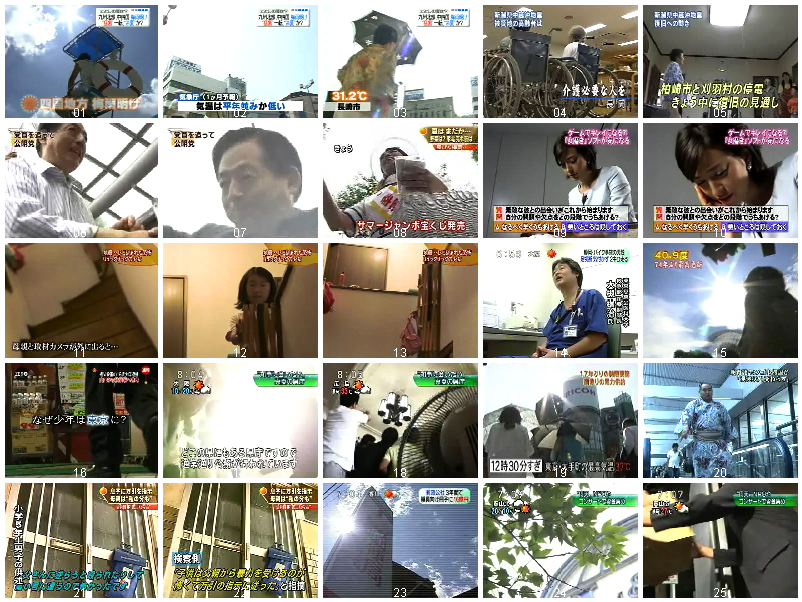
\includegraphics[width=14cm]{lowanglemontage.jpg} 
   \caption[Very low-angle images]{The 25 cuts which used a very low camera angle.}
   \label{fig:lowanglemontage}
\end{figure}

The images shown in fig.\ref{fig:lowanglemontage} illustrate the diversity of images found in the corpus and hint at the diversity of motivations behind the camera operators decision to portray the subject from the chosen angle. These images can be divided into three broad groups based on a consideration of various aspects of the actual circumstances within which the image was created; 

\begin{description}
\item [Positional Motivation] Images of objects or people where the camera operator is unable, because of the limitations of time and physical surroundings, to be on the same level as the object. For example, image 1 in fig.\ref{fig:lowanglemontage} which shows a swimming pool lifeguard in an elevated chair, or images 11--13 which show a young girl, deeply worried by the recent earthquake, at the top of the stairs of the family home after getting out of bed to seek reassurance from her mother. Image 7 shows the leader of the Komeito political party, Ota Hiroaki, addressing a crowd of supporters from the top of a campaign bus. As is often the case in Japanese political campaigning, the vehicle used is fairly small and there would be little room for a camera operator as well as the candidate even if permission to shoot from the roof of the bus could be gained from the Komeito organisers, thus the pictures are from ground-level.\footnote{Of course, not knowing the details of the shoot we cannot know whether there was a \emph{conscious decision} to prefer a ground-level view to an available alternative or whether this position was the only one accessible.}

\item [Relational Motivation] These images attempt to illustrate not the objects or social actors portrayed but concentrate on the relationship between them. Thus we have several shots (2, 3, 15 \& 19) which show `people under the sun', that is ordinary people suffering the effects of very hot summer weather. In these images it is not the sky or the sun that is the object of interest, nor is it the passers-by as individual, it is the shared condition of being human in temperatures of 40 degrees and more.

A related image is number 18, this shows the relationship between a group of tourists, waiting in the sweltering summer heat in the town hall of Miyazaki Prefecture in the south of Japan to catch a glimpse of celebrity mayor Higashikokubaru Hideo, with the small fan placed on the floor in the foyer of the building. The fan is significant in this instance as it symbolises the money-saving activities of Higashikokubaru's administration who have decided to turn off the building's air-conditioning despite the high temperatures.

Image 5 shows (or purports to show) the moment electricity is restored to a family home after being cut off in the wake of an earthquake. The return of power is illustrated by the family gathering in the the home's main room for  mother to switch the light, on the ceiling, on. The important elements here can be seen to be the family, including the children and the illuminated electric light fitting. Perhaps if the home had been lit by table-lamps the image producer would have portrayed the scene differently.
\item [Technical Motivation] Image 23 shows the exterior sign-board of a post-office. The sign-board is considerably taller than it is broad and very different in shape to the 4:3 camera frame. The image producer here has found a way of reconciling the two shapes by means of foreshortening. Placing the camera lens near the base of the sign allows the camera-operator to create a framing which includes the whole of the sign. 

However, it should be noted that in this case alternatives exist;
\begin{close_enum}
\item the image-maker could have chosen a tilt (a vertical camera move) that took in all of the signboard, or  
\item the image-maker could have moved away from the sign-board allowing it to fit within the frame of a stationary shot.
\end{close_enum}

The decision to prefer the low-angle shot was taken by the camera operator and only he/she can know why it was made. It seems not unreasonable to apportion a degree of influence to the attitude of the story in which it appears. This story is critical of the Japanese Post Office for spending tax-money on internal publications which, the story argues, no-one reads and are thus a waste of resources. The Post Office is portrayed as a threatening presence gobbling up tax-yen for its own private purposes, it may have been a desire to hint at this sense of threat that motivated the camera-operator to prefer this way of shooting the sign to the alternatives.
\end{description}

Most of the low-angle shots we come across in news are in some part under the influence one or more of the motivations above, but there are some examples in the corpus (including possible the image of the Post Office signboard just mentioned) where the conventional association of low-camera angle with subject empowerment might be posited as being a factor. However, these images are in the minority.

\bigskip

Image 6 shows a senior politician, Ota Akihiro of the Komeito\index{Komeito} (Clean Government Party) shaking hands with supporters at an outdoor rally. Why has the camera operator chosen to capture this particular image? We might put it down to the fact that the individual portrayed is a powerful politician and the image-maker is choosing, through the choice to mobilise the semiotic resource of the low camera angle, to make him seem more imposing. However, looking at the whole 3.9 seconds duration of the image, it seems more likely that this was an attempt to foreground the hand-shaking between Ota and the crowd, putting the camera below the level of the outstretched hands to include them in the image along with Ota.\footnote{One of the camera operators interviewed in Tuchman (1973:8)\nocite{Tuchman:1973} criticises what sounds from the description to be a similar low-angle shot of US politician Adlai Stevenson as the camera operator has emphasised the hand-shaking at the expense a clear view of the individual's face.} 

Nevertheless, we are left with the fact that the image, whatever the motivation which led to its creation in this particular form, was chosen for use in the final broadcast version of the story. That it was not rejected because of its potential semiotic content --- the implication of a relationship of power-subordination between powerful portrayed (politician) and subjected viewer (voter) --- can be seen as either indicating an insensitivity to, or lack of understanding of this potential meaning of the image, or, a collective acknowledgement that this image, with all its semiotic implications, is appropriate in this context. 

This story consists of 28 cuts, 21 of these cuts portray Mr Ota who is on screen for 3:12 of the total 3:52 duration of the story. Such prominence given to a single individual, along with the fact that we are told he is leader of a political party, would seem to make the relatively weak visual communication of one image shot from a low-angle almost superfluous. During the course of the story he is portrayed from a high or very high angle six times and from a low or very low angle three times. If we attribute to these cuts their conventional semiotic reading we should conclude that Ota is portrayed overall as being in a rather less powerful position as regards the viewer. As a politician, a `public servant' we could indeed argue that this is an accurate reflection of his actual position, however the mere fact of the duration of his exposure seems to argue in the other direction. It can be seen that the various portrayals shown in the story, if given their traditional semiotic interpretations, do not add up to a consistent statement about the individual portrayed, and it is difficult to conclude that the images `tell' us anything about him.

\bigskip
Image 8 which shows a young woman handing out promotional packs of tissues. The event she is promoting is the sale of tickets for the yearly `Summer Jumbo' lottery. Similar motivations to those mentioned above, the foregrounding of the action of the hands, the association of the lottery with the sunny skies and high temperatures of summer, seem to be behind this image. This is more an image which attempts an economical depiction of an action, the handing out of packs of tissues, in a situational context meaningful to the audience, than a portrayal of a unique social actor.

We are then left with images 14, a doctor wearing a blue uniform, and 20, sumo-wrestler Asashoryu walking through an airport. The doctor, who is interviewed during the course of the story, is portrayed in typical interview shot (MCU, camera at eye-level, half-profile), it is only this cut, over which the narrator introduces him as a doctor with `twenty years experience in emergency medicine' in order to validate the conjectures he is about to be shown making. Perhaps the camera operator intended to contribute to this validation of the portrayed individual as an `authority' by creating this image. If this is the case then we might be able to point to this image as an example of the use of the low angle shot as an indicator of authority; there is, in this case, to be no other particular motivation for the choice of this angle, there seems to be no particular merit in including more of the ceiling of the consultation room in the shot, the doctor's immobile hands are of no particular interest in this shot, the camera operator is not trying calling out attention to a particular spatial relationship, the low angle does not afford a better view of the doctor's face and he is seated at the same level as the camera operator and reporter.

Even if the motivation was mere playfulness on the part of the camera operator or the desire to capture a `different' image to those which typically make up the standard interview, we must acknowledge the fact that he or she chose a low angle over any other type of shot and that this was again chosen (in preference to what we do not know, not having the original camera recording available) by the editor as a suitable image to go with the narration. It  would be going too far to say that the camera operator and editor pro-actively chose to mobilise the semiotic resource of the low angle `empowering' shot to portray the doctor (who is also deputy section-chief (\emph{fuku-buch\-{o}} \cjk{副部長}) at a medical school and thus has considerable social status), but the image's appearance in the story as broadcast indicates that it was allowed to pass through the various gatekeepers who filter news content and was deemed at every stage appropriate, or at least, not \textit{in}appropriate.

\subsubsection{Low-angle shots and non-human images}\label{subsubsec:nonhum}

In this short section I look briefly at two uses of low angle shots regularly used in the portrayal of certain inanimate objects. This is admittedly a departure from my focus on the portrayals of human social actors but, as I will show, these sorts of images begin to approach a repeatable form that can be identified as a typical feature of stories of a particular type. 

\paragraph{`Crime Doors'}
A specific and consistent use of the very low angle portrayals is as an indicator of some connection of a home or other building with crime or behaviour which has or may have violated law or social mores.

\begin{figure}[t]
\centering
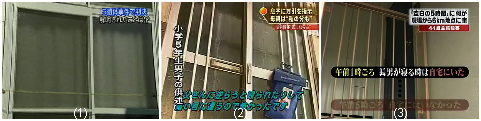
\includegraphics[height=2.5cm]{crimedoors.jpg} 
\caption{House and apartment doors connected with crime}
\label{fig:crimedoors}
\end{figure}

The three images in figure \ref{fig:crimedoors} are taken from stories which deal with (1) a multiple murder, (2) child abuse and shoplifting and (3) another murder. The doors portrayed are the family homes of those involved in the various crimes, either those of the victims or of the alleged perpetrator, or in the case of the first story which covered the arrest of a mother suspected of involvement in the suspicious deaths of three of her own children, both. As can be seen they all choose to portray the door in question from a low angle, giving a very different view to the one an adult observer would be used to.

The regular depiction of doors in this way, they are almost a visual clich\'{e}, might be attributable to two very different factors. First we take into account the shape that doors take, they tend to be the correct shape for an adult human to pass through standing up, that is, tall and thin, or for the double doors common in Japan, roughly square. A television screen on the other hand is, relatively speaking, short and broad. The low-angle shot may be an attempt to include as much of the door in one shot by making use of the visual foreshortening that occurs when we view an object from near one of its extremities. However, a look at the images presented in figure \ref{fig:crimedoors} suggests that this is not the reason: if the camera operator had wanted an image of the whole door, why not take a few steps back? why not move to the side?

An interpretation in line with the conventional wisdom of semiotic theory seems to be valid in the case of `crime doors'. The viewer is placed in a position of powerlessness, with regards to not just this crime, but to the social fact of crime. However, whether the decision to create such images is the result of specific training, of an unconscious mimicking of previous images of crime-scene doors, a conscious desire on the part of the image-maker to create an image of `fear', or the desire to emphasise danger and heighten the \textit{frisson} in coming close to it, it is impossible to say from the data this study has access to. 

Doors act simultaneously as both a defence against the unknown contained within and as a possible connection with that unknown. Were the door to be opened we would catch a glimpse of what we might suspect, but do not know, has happened, but we would also prefer the crime the room has (or may have) contained to remain safely within. Jobes (1961:463)\nocite{Jobes:1961}, whose interpretations are derived from art historical tradition rather than empirical study, suggests that the door is used as a symbol of defence, protection and revelation, also as a barrier and marker of secrets and separation.\footnote{Similar interpretations can be found in de~Vries (1974) and Leach (1972).\nocite{Leach:1972} \nocite{Vries:1974}} 

\paragraph{`Official Windows'}
Official statements, actions and decisions reported by news media may be attributed not to individual speakers but more generally to the bodies or organisations which issue them. For example, a story about the overseas trial of a Briton might be attributed to `the Foreign Office', the announcement of a possible change in policy might be prefixed by the words ` ministry sources revealed'. Where the  source of information is a body rather than an individual it is not uncommon for images of the official seat of that body to be used as a visual proxy for the individual bureaucrat, spokesperson or press-officer who may actually have been the source of the information. 

\begin{figure}
\centering
\includegraphics[height=2.5cm]{windows.jpg} 
\caption{Official buildings' windows as proxy actors}
\label{mont:windows}
\end{figure}

This practise is certainly familiar to viewers of television in the UK as well and is not particularly noteworthy in itself. However, what interest me here is the low angle depiction chosen by the image-makers in a number of the instances of this kind of image found in the corpus (fig.\ref{mont:windows}). Each of the buildings depicted here has windows on its ground floor, images of which would have been still have been adequate images of the windows of the building in question. Instead, the choice has been made to prefer images of windows higher up the building, thus increasing the amount of looking up we, as viewers, have to do. This also has the effect of increasing the feeling of physical separation between viewer, stuck on the ground, and those who occupy the spaces hinted at by the windows. I would argue this may contribute to an exaggerated impression of the loftiness of officialdom, whether we attribute this to a media critical of the power of the bureaucracy who therefore create images which place the viewer in a position similar to the one they adopt, or a desire to reflect accurately the considerable influence of bureaucrats in Japanese society.

\subsection{High-angle shots: visual access}
The primary motivation behind the use of high-angle shots, rather than to express any relationship of power or subjection seems to be the fact that a higher viewpoint gives a broader view of an area. As can be seen in the images shown in figure\ref{fig:montage-hiang}, the primary subject matter is `crowds' and `groups'. These images show; 

\begin{close_enum}
\item a group of trawler workers loading a catch
\item a crowd of rescue workers and onlookers attempting to rescue an earthquake victim
\item a team of demolition workers pulling down the remains of a quake-damaged property
\item Komeito leader Ota Akihiro surrounded by helpers and voters
\item a group of policemen searching for evidence near the scene of a murder (taken from a helicopter)
\item a retired man discussing his pension with local government adviser
\item members of a committee dealing with pension record problems entering a meeting hall
\item shoppers inside a large hall
\item a temp-agency `whistle-blower'
\end{close_enum}

\begin{figure}[t]
\centering
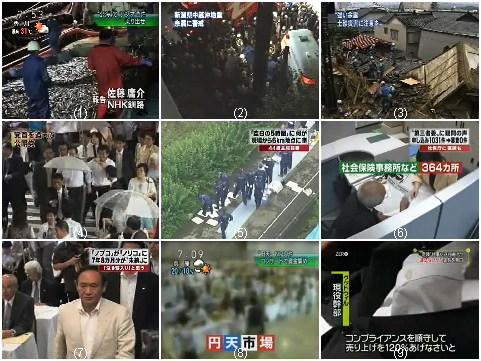
\includegraphics[width=10cm]{hiAngle-montage.jpg} 
\caption[Montage of high-angle camera shots]{Nine of the ten very high-angle shots found in the corpus.}
\label{fig:montage-hiang}
\end{figure}

The angle chosen by the image-maker in these scenes (fig.\ref{fig:montage-hiang}) has very little to do with the desire to show the portrayed actors as being somehow powerless or in a position of subordination and everything to do with getting a good `overview' of a scene which plays out on the flat, providing an adequate and economical visual description of the physical space within which the portrayed events or actions are taking place. This view is supported by framing data drawn from the corpus, 70 per cent of the very high-angle images are also in VLS (very long shot) or LS (long shot), for eye-level depictions the proportion is much lower at just 16 per cent (see fig.\ref{fig:framvang}). While counts for very high-angle shots (\emph{n}=10) are too low to allow categorical statements on the matter, the corpus data does offer some support for the argument that the very high angle shot, which is, as often as not, a wide or very wide shot, is used primarily as a way of conveniently capturing and depicting the scale of events occurring on a fairly wide stage rather than as a semiotic resource expressing, or putting forward, the image-maker's view of the power relationship which should obtain between the portrayed and the image-maker or audience.

This can be seen as an attempt on the part of the image-maker to avoid dissonance between image and narration. Such dissonance can  have an effect on audience understanding \citep{Grimes:1991}. If, for example, the news report is of a political rally which, accurately or not the commentary tells us, that ten thousand people attended and the image-maker brings back a selection of images from the rally shot from in front of the crowd and thus showing just the front `layer' of participants, this would lead us to question the accuracy of the reported figures. If ten thousand people attended why not show them? Why show just 150? The most convincing shot the image-maker could bring back, that shot most consonant with the claims of the commentary, would be that which showed, in an instant, every one of the ten thousand reported attendees; such an image cannot be taken from eye level unless the event takes place in an amphitheatre or other space specifically designed to create an eye-line between a given point and a large number of viewers/objects. The simplest strategy in the absence of the above is for the image-maker to seek some raised vantage point from which such a view can be obtained.

Some distinction must be made between high-angle wide shots, which can be considered semiotically innocuous in the sense that they are, I would argue, not the result of an intention to depict power relations but to depict scale, and high-angle shots at tighter framing sizes, which may well have a different intent. 

\begin{filecontents*}{fram-vang.csv}
v.low, low, eye-level, high, v.high
14.3, 56.8, 57.1, 42.0, 10.0
71.4, 28.4, 26.4, 29.5, 20.0
14.3, 14.8, 16.5, 28.4, 70.0
\end{filecontents*}
\begin{figure}[t]
\centering
\psset{xunit=1.7cm,yunit=.04cm} 
\newpsbarstyle{lgray}{fillstyle=solid, fillcolor=lightgray, linecolor=darkgray, linewidth=0.5pt}
\newpsbarstyle{ggray}{fillstyle=solid, fillcolor=gray, linecolor=darkgray, linewidth=0.5pt}
\newpsbarstyle{dgray}{fillstyle=solid, fillcolor=darkgray, linecolor=darkgray, linewidth=0.5pt}
\begin{pspicture}(0,-30)(6,110)%sets page size in 5mm units
\psaxes[linecolor=gray,tickstyle=top, ticksize=0.01, axesstyle=axes,Ox=0,Dx=1,Dy=20, labels=y, ticks=y](0,0)(5,100)
\readpsbardata{\data}{fram-vang.csv}%gets data from file
\psbarchart[chartstyle=stack, barstyle={dgray, ggray, lgray}, barcolsep=0.5, barlabelrot=90]{\data}%
\rput[l](5,80){\textsc{LS+VLS}}
\rput[l](5,20){\textsc{MS+MLS}}
\rput[l](5,5){\textsc{VCU+CU+MCU}}
\rput[r](-0.5,50){\%}
\end{pspicture} 
\caption{Distribution of framing sizes by vertical camera angle}
\label{fig:framvang}
\end{figure}

\medskip

If we accept the coincidence of high camera angle with the need to produce an image of broad visual scope, then, of the images presented in fig.\ref{fig:montage-hiang}, only images 6 and 9 seem to be in need of further consideration. 

Image 6 shows an elderly man in conversation with a local government pension adviser, between them on the desk can be seen a small paper sign which tells us the exact role of the adviser on the right of the image. The shot in its entirety is a zoom-out which starts on a close-up of this sign and rapidly widens to show the scene depicted here. The motivation for this shot therefore seems to be rather the wish to make the image as informative as possible by including the written information of the sign, possibly only clearly visible to the camera from this unusual angle.

\medskip

Image 9 is unusual in that its intention is to prove the existence of the individual portrayed without identifying them. This image is taken from a 3:22 story concerning the activities of the Goodwill temp agency. In Japan, these agencies are limited in which types of employment they can offer to those who register with them, prohibited areas of work include `security'(\textit{g\={a}doman}) and construction. In 2006 Goodwill were discovered to have provided people for this type of work and were found to have engaged in the illegal practise of `double dispatch' where temporary workers are sent to a subcontracting temp agency which then dispatches them on. Goodwill Group's labour and staffing agency arm ceased to exist in July 2008 after its business licence was revoked by the Ministry of Health, Labor and Welfare.\footnote{\textit{The Japan Times}, `Goodwill pulls plug on temp agency', 1 Aug 2008. \newline Online: \url{search.japantimes.co.jp/cgi-bin/nn20080801a5.html} - 4 Jul 2009} The individual portrayed throughout this story is a Goodwill employee, we are shown part of his business card (\textit{meishi} \cjk{名刺}) and the camera focuses on his company badge repeatedly, speaking about Goodwill's illegal activities in the branch offices he manages.

The shot shown in fig.\ref{fig:montage-hiang}(Image 9) looks downward, into his lap where his hands rest, from over his left shoulder. It may seem facile to suggest this but I would argue that the most likely reason for the particular from this image takes is that the camera operator had run out of other options and was trying to keep the interview visually interesting. This cut occurs toward the end of the piece at a point where the more natural shots have already been taken. In the `normal' interview where the speaker is shown speaking, the camera operator has little choice but to maintain a fairly steady shot of the speaker's face; in this situation, this is exactly what is prohibited and some alternative yet meaningful image must be created. A man seated in a semi-darkened room wearing a dark suit and white shirt presents little in the way of grist for the creative mill and this particular image creator seems to have chosen to vary the position and angle of the camera as a surrogate for what we normally expect to see, the changing expressions and attitude of the speaker.

\subsection{Summary}
In very few of the very high or low angle images found in the corpus does an interpretation based solely on the supposedly `subordinating' or `empowering' nature of these shots seem appropriate, given what we know of the circumstances of production. The images which make use of these `semiotic resources' would be, in the majority of cases, difficult to account for in terms of any intention on the part of the image-maker to communicate the meaning which can be inferred. 

For the purposes of this study the evidence we have to draw on is the texts themselves and conclusions cannot be based  on what \textit{may} have been going through the mind of the image-maker or how a viewer \textit{might} read the image, the only way forward is to survey the images as used, identify consistencies and suggest explanations for the patterns of use identified. Variations in vertical camera angle can be seen to be more connected to the image-makers desire to provide a succinct depiction of a given object or relationship of a certain size or scope, whether this a politician on a `meet and greet' or a crowd of demonstrators. If the flow of images of television news is to be viewed as a form of communication then it must also be admitted that this stream of information is heavily motivated by ideational considerations and a need for parsimony of realisation. Any interpersonal meanings, any assessments or evaluations of relationship between the portrayed and the viewer seem to be very secondary.
\printbibliography

\end{document}